\documentclass[aspectratio=169]{beamer}

% ============================================================
% 10-MINUTE TALK + 5-MINUTE Q&A BACKUP   (visual, minimal text)
% Two speakers: Jasmin (slides 1-6) / Daniel (slides 7-11).
% The words live in SPEAKER_SCRIPT_10min.md; slides are visual cues.
% ============================================================

\usepackage{tikz}
\usepackage{amssymb}
\usepackage{booktabs}
\usepackage[T1]{fontenc}
\usepackage[utf8]{inputenc}
\usepackage{graphicx}
\usepackage{hyperref}
\usetikzlibrary{arrows.meta, positioning, calc, backgrounds}

\usetheme{metropolis}
\metroset{numbering=none, progressbar=foot, block=fill, sectionpage=none}

% ---- palette --------------------------------------------------------------
\definecolor{ink}{HTML}{20303A}
\definecolor{accent}{HTML}{2D9CDB}
\definecolor{accentdk}{HTML}{1B6FA8}
\definecolor{warm}{HTML}{E07A3F}
\definecolor{good}{HTML}{3DA35D}
\definecolor{faint}{HTML}{C9D3DA}
\definecolor{paper}{HTML}{FBFCFD}

\setbeamercolor{normal text}{fg=ink, bg=paper}
\setbeamercolor{frametitle}{fg=paper, bg=ink}
\setbeamercolor{alerted text}{fg=accentdk}
\setbeamercolor{progress bar}{fg=accent, bg=faint}
\setbeamerfont{frametitle}{size=\large}

% ---- helpers (names chosen NOT to clash with LaTeX builtins) --------------
\newcommand{\bignum}[2]{{\fontsize{34}{36}\selectfont\textbf{#1}}\\[2pt]{\footnotesize\color{ink!70}#2}}
\newcommand{\lab}[1]{{\footnotesize\color{ink!65}#1}}

\title{Can you trust a verification tool you rewrote yourself?}
\author{Jasmin Begi\'{c} \quad$\cdot$\quad Daniel Wassie}
\institute{Advanced Systems Engineering --- University of Salzburg}
\date{June 24, 2026}

\begin{document}

% =====================================================================
% 1 . TITLE
% =====================================================================
{\setbeamercolor{background canvas}{bg=ink}
 \setbeamercolor{normal text}{fg=paper}
\begin{frame}
  \vfill
  \centering
  {\fontsize{25}{29}\selectfont\textbf{\textcolor{paper}{Can you trust a verification tool}}}\\[3pt]
  {\fontsize{25}{29}\selectfont\textbf{\textcolor{paper}{you rewrote }\textcolor{accent}{yourself}\textcolor{paper}{?}}}\\[1.4em]
  {\normalsize\color{faint}Rotor in Rust --- faster, wider, readable.}\\[2.2em]
  {\small\textcolor{paper}{Jasmin Begi\'{c}}\quad$\cdot$\quad\textcolor{paper}{Daniel Wassie}}\\[0.4em]
  {\footnotesize\color{faint}Advanced Systems Engineering --- supervised by Christoph Kirsch}
  \vfill
\end{frame}}

% =====================================================================
% 2 . THE PROBLEM                                              [JASMIN]
% =====================================================================
\begin{frame}{You cannot test every input}
  \vfill
  \centering
  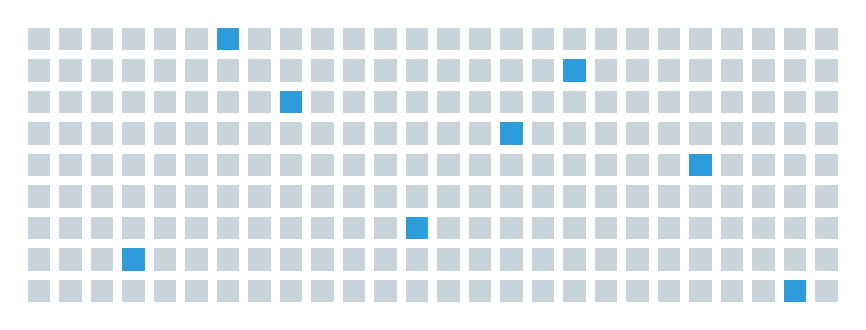
\begin{tikzpicture}[x=0.40cm, y=0.40cm]
    \foreach \x in {0,...,25}{
      \foreach \y in {0,...,8}{
        \fill[faint] (\x,\y) rectangle ++(0.72,0.72);
      }}
    \foreach \p in {(3,1),(8,6),(12,2),(17,7),(21,4),(24,0),(6,8),(15,5)}{
      \fill[accent] \p rectangle ++(0.72,0.72);
    }
  \end{tikzpicture}
  \vfill
  {\large 8 bytes of input $=\;2^{64}$ possibilities.}\\[4pt]
  \lab{Testing samples a few (\textcolor{accent}{blue}). The crash can hide
       anywhere in the grey.}
  \vfill
\end{frame}

% =====================================================================
% 3 . THE IDEA                                                 [JASMIN]
% =====================================================================
\begin{frame}{Verification asks one question --- for all of them}
  \vfill
  \centering
  {\large Can it reach a bad state within $k$ steps, for \alert{any} input?}
  \vfill
  \begin{columns}[T]
    \column{0.46\linewidth}\centering
      \textbf{Yes} $\;\rightarrow$ the exact input that does it
    \column{0.46\linewidth}\centering
      \textbf{No} $\;\rightarrow$ a guarantee, up to $k$
  \end{columns}
  \vfill
  \lab{The unknown input is treated as algebra, not as guesses.}
\end{frame}

% =====================================================================
% 4 . THE PIPELINE                                             [JASMIN]
% =====================================================================
\begin{frame}{Our tool turns a real binary into that question}
  \vfill
  \centering
  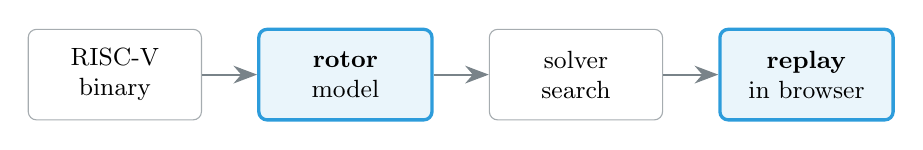
\begin{tikzpicture}[
      box/.style={draw=ink!40, rounded corners=3pt, minimum height=1.15cm,
                  minimum width=2.2cm, align=center, font=\small},
      ours/.style={box, draw=accent, fill=accent!10, very thick},
      arr/.style={-{Stealth[length=3mm]}, ink!60, thick}]
    \node[box]                       (bin) {RISC-V\\binary};
    \node[ours, right=0.7cm of bin]  (mod) {\textbf{rotor}\\model};
    \node[box,  right=0.7cm of mod]  (sol) {solver\\search};
    \node[ours, right=0.7cm of sol]  (vis) {\textbf{replay}\\in browser};
    \draw[arr] (bin)--(mod); \draw[arr] (mod)--(sol); \draw[arr] (sol)--(vis);
  \end{tikzpicture}
  \vfill
  \lab{Rotor existed --- one 14{,}000-line C file. We rebuilt it (blue), and
       added the last step.}
\end{frame}

% =====================================================================
% 5 . SPEED                                                    [JASMIN]
% =====================================================================
\begin{frame}{The rewrite ran three orders of magnitude faster}
  \vfill
  \centering
  \begin{columns}[c]
    \column{0.5\linewidth}\centering
      \lab{TIME}\\[6pt]
      {\large\color{warm}139\,s}\;{\large$\rightarrow$}\;\bignum{0.1\,s}{}
    \column{0.5\linewidth}\centering
      \lab{MEMORY}\\[6pt]
      {\large\color{warm}428\,MB}\;{\large$\rightarrow$}\;\bignum{20\,MB}{}
  \end{columns}
  \vfill
  \begin{center}\small
  One question --- \emph{``built this piece before?''} --- answered two ways:\\[4pt]
  \textcolor{warm}{11{,}695{,}232{,}963} list comparisons \quad vs.\quad
  \textcolor{accent}{\textbf{159{,}018}} hash lookups.
  \end{center}
  \vfill
\end{frame}

% =====================================================================
% 6 . EQUIVALENCE                                     [JASMIN -> hands off]
% =====================================================================
{\setbeamercolor{background canvas}{bg=good!10}
\begin{frame}{Faster is worthless if it is wrong}
  \vfill
  \centering
  {\fontsize{80}{82}\selectfont\textbf{\color{good!55!black}36 / 36}}\\[10pt]
  {\large the same bug, at the \alert{same step}, in both tools}\\[4pt]
  \lab{18 programs $\times$ 2 settings --- the solver itself is the referee.}
  \vfill
  \lab{The step number fingerprints the whole run; one wrong instruction
       shifts it.}
\end{frame}}

% =====================================================================
% 7 . SYMBOLIC ARGV                                            [DANIEL]
% =====================================================================
\begin{frame}{A whole class of bugs was unreachable}
  \vfill
  \begin{columns}[c]
    \column{0.5\linewidth}\centering
      \lab{BEFORE}\\[8pt]
      {\large\ttfamily ./prog \textcolor{faint}{??????}}\\[8pt]
      {\footnotesize Arguments were \textbf{frozen}.}
    \column{0.5\linewidth}\centering
      \lab{NOW}\\[8pt]
      {\large\ttfamily ./prog \textcolor{accent}{\textbf{??????}}}\\[8pt]
      {\footnotesize The solver fills the \textbf{open} bytes.}
  \end{columns}
  \vfill
  \centering\lab{Listed as ``future work'' in the original paper. We built it.}
  \vfill
\end{frame}

% =====================================================================
% 8 . THE X / Y BUG                                            [DANIEL]
% =====================================================================
\begin{frame}{The solver discovers the secret by itself}
  \vfill
  \centering
  \colorbox{ink}{\color{paper}\large\ttfamily\;if (arg1[0]=='X' \&\& arg2[0]=='Y')\;\textcolor{warm}{crash}\;}
  \vfill
  {\large Two letters, in \alert{two different} arguments, at once.}\\[4pt]
  \lab{Unreachable from the keyboard --- the program never reads it.}
  \vfill
  {\large Solver, in seconds:\quad
   {\ttfamily arg1[0]=\textcolor{accent}{\textbf{X}}}\quad
   {\ttfamily arg2[0]=\textcolor{accent}{\textbf{Y}}}}
  \vfill
\end{frame}

% =====================================================================
% 9 . VISUALIZER (screenshot, not live)                        [DANIEL]
% =====================================================================
\begin{frame}{The answer, made watchable}
  \vfill
  \begin{columns}[c]
    \column{0.46\linewidth}\centering
      \fbox{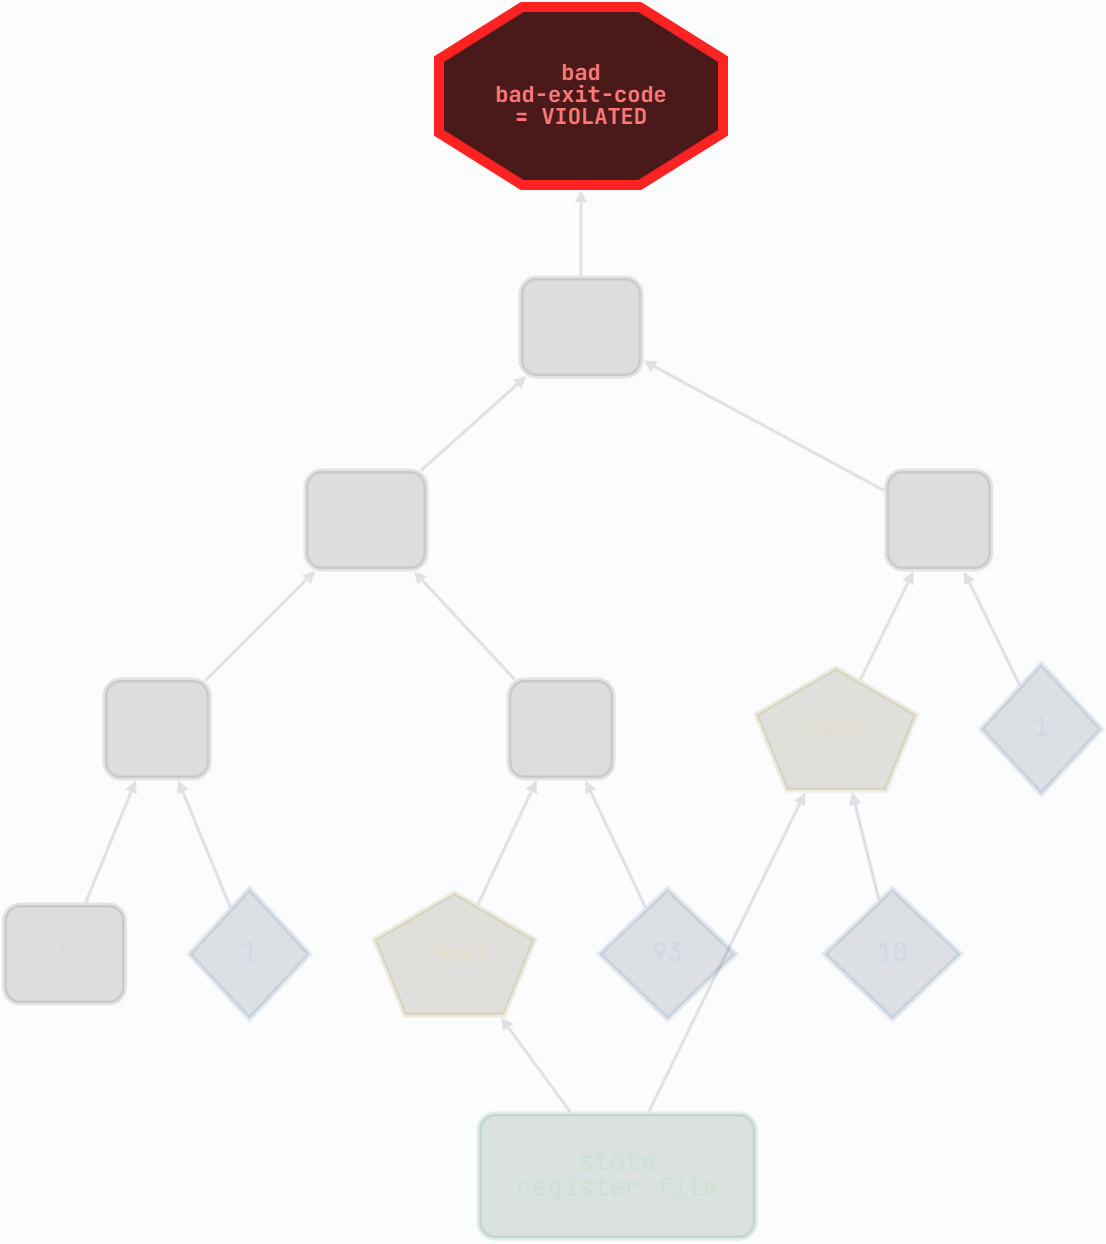
\includegraphics[height=0.68\textheight]{figures/visualizer_graph.png}}
    \column{0.5\linewidth}
      The witness replayed in the browser. At the final step the bad
      state --- \textcolor{warm}{\textbf{bad-exit-code VIOLATED}} ---
      lights up red, fed by the logic that read the argument bytes.\\[1em]
      \lab{Live tool, 12 examples: jaspek.github.io/rotor-rust}
  \end{columns}
  \vfill
\end{frame}

% =====================================================================
% 10 . THE TWIST                                               [DANIEL]
% =====================================================================
\begin{frame}{The speed was one idea --- so we proved it in C too}
  \vfill
  \centering
  \begin{columns}[t]
    \column{0.33\linewidth}\centering\bignum{95$\times$}{faster, in the original C}
    \column{0.33\linewidth}\centering\bignum{0}{lines of output changed}
    \column{0.33\linewidth}\centering\bignum{36/36}{still equivalent}
  \end{columns}
  \vfill
  \lab{Not the language --- one data structure. The hard part of a rewrite is
       proving it still tells the truth.}
  \vfill
\end{frame}

% =====================================================================
% 11 . CLOSE
% =====================================================================
\begin{frame}[standout]
  Thank you.\\[0.6em]
  {\small $1000\times$ faster \;$\cdot$\; a new class of bugs reachable
   \;$\cdot$\; 36/36 verified \;$\cdot$\; readable answers}
\end{frame}

% =====================================================================
% =================  BACKUP --- Q&A MATERIAL  ==========================
% =====================================================================
\begin{frame}{Backup: the counting, in full}
  \centering\footnotesize
  \begin{tabular}{lrr}
    \toprule
     & C rotor & Rust rotor\\
    \midrule
    Node creations           & 3{,}171{,}632 & 159{,}018\\
    Dedup question asked      & 9{,}976       & 159{,}018\\
    Hits (already present)    & 6{,}021       & 48{,}114\\
    \textbf{Basic operations} & \textbf{11{,}695{,}232{,}963} & \textbf{159{,}018}\\
    \bottomrule
  \end{tabular}\\[0.6em]
  \lab{Self-check: creations $-$ hits $=$ each tool's own reported line count,
       exactly.}
\end{frame}

\begin{frame}{Backup: Rust vs.\ the optimized C}
  \centering\footnotesize
  \begin{tabular}{lrrr}
    \toprule
    selfie model & baseline C & C + hash & Rust\\
    \midrule
    Time          & 139\,s  & 1.5\,s  & $<$0.1\,s\\
    Memory        & 428\,MB & 485\,MB & 20\,MB\\
    Lines created & 3.17\,M & 3.17\,M & 159\,k\\
    \bottomrule
  \end{tabular}\\[0.6em]
  \lab{The hash fixed the lookup. Rust also never \emph{creates} the
       duplicates; C still does, then prunes.}
\end{frame}

\begin{frame}{Backup: disabling deduplication in both}
  \begin{itemize}\setlength\itemsep{0.5em}
    \item C rotor: \textbf{crashes} (\texttt{ite then sort mismatch}). Line
          reuse there is load-bearing, not just speed.
    \item Rust (\texttt{-{}-no-cse}): runs; model grows 1.4$\times$;
          \emph{identical} solver verdict.
    \item Deduplication changes size and speed --- never meaning.
  \end{itemize}
\end{frame}

\begin{frame}{Backup: why the file sizes differ}
  \centering\footnotesize
  \begin{tabular}{lrr}
    \toprule
    selfie model & with comments & comments stripped\\
    \midrule
    C rotor    & 10.6\,MB & 5.2\,MB \;(50.8\% was comments)\\
    Rust rotor & 3.1\,MB  & 3.0\,MB\\
    \bottomrule
  \end{tabular}\\[0.6em]
  \lab{Same content, different spelling: comments, binary vs decimal
       constants, longer node numbers. Meaning is identical.}
\end{frame}

\begin{frame}{Backup: how symbolic argv works}
  \begin{itemize}\setlength\itemsep{0.45em}
    \item Argument bytes $=$ \textbf{uninitialized model states} --- the
          paper's own device for input; the rest of the stack is concrete.
    \item The program reads them through ordinary loads --- decoder, memory,
          and checks all untouched.
    \item Scope: argument \emph{count} fixed, lengths bounded; we explore
          \emph{content}. Sound for C-string programs.
  \end{itemize}
\end{frame}

\begin{frame}{Backup: what we do \emph{not} claim}
  \begin{itemize}\setlength\itemsep{0.45em}
    \item Not a formal proof of generator equivalence --- undecidable, and the
          paper's own future work.
    \item Evidence is bounded: 18 programs, depth 1500, two settings.
    \item Two benchmarks agree only by both finding nothing --- weaker than a
          step-exact match.
    \item One anomaly was \emph{our harness}, not the rotor; we caught it
          because one row disagreed with seventeen.
  \end{itemize}
\end{frame}

\end{document}
